\begin{appendices}
\chapter{Proofs of Chapter \ref{chp:4}} \label{app:chap4}

This section discuss if the chosen estimators prensented in Chapter \ref{app:chap4} have satisfying proprieties in the context of left censored data. This section consists in verifying all the conditions and hypothesis needed to ensure the convergence of our chosen estimators. First, we check if $\hat \lambda$ esti-
mated with the Newton-Raphson procedure converges to $\lambda^*$. Then, we will follow the same demonstration than \cite{Lavielle1997} to proove that the left censorship does not hinder the convergence of the breakpoint estimators $\hat K$ and $\hat t$. Lastly, we will check if the necessary conditions to use the PELT algorithm are verified. 

\section{On the convergence of \texorpdfstring{$\hat\lambda$}{l}}

We managed to find a computational way to treat samples where all measurements are censored. In that case, the maximum is reached when $\lambda$ tends to infinity (there is no convergence) and the cost function tends to 0. In our algorithm, the value of $\hat\lambda$ is upper bounded by a $\lambda_{max} = 10^6$.   
We are interested in the other case where there are some non censored observations. The scale estimator $\hat\lambda$ is estimated using Newton-Raphson. The convergence hypothesis stated in \textit{Theorem 1} of \cite{Verbeke1995} are hard to verify given the formula of the function to be maximized. Since we are looking for the maximum of Equation \ref{eq:ml-wei-1}, it implies to find the zero of Equation \ref{eq:ml-wei-d1}. We can rewrite this equation : 

\begin{equation}\label{eq:ml-wei-d1-bis}
\frac{\partial\sum_{i=t_{k}+1}^{t_{k+1}}\ln f(y;\lambda,\sigma)}{\partial \lambda} = n_a\frac{a^\sigma\sigma(\lambda)^{\sigma-1}e^{-(\lambda a)^\sigma}}{1-e^{-(\lambda a)^\sigma}} + (n_{seg}-n_a)\frac{\sigma}{\lambda} - \sigma(\lambda)^{\sigma-1}\sum_{i \notin \mathcal{N}_a}y_i^{\sigma}, 
\end{equation}
with $n_{seg}$ being the number of observations in segment $t_{k}+1:t_{k+1}$ and $n_a$ its number of censored observations. We will denote \ref{eq:ml-wei-d1-bis} by $\partial\mathcal{L}(\lambda;y,\sigma)$ to simplify the notations. We can then compute the second derivative that can be written : 

\begin{align}\label{eq:ml-wei-d2-bis}
\begin{split}
\frac{\partial^2\sum_{i=t_{k}+1}^{t_{k+1}}\ln f(y;\lambda,\sigma)}{\partial \lambda^2} =  n_a&\frac{a^\sigma\sigma(\sigma-1)\lambda^{\sigma-2}e^{-(a\lambda)^\sigma}}{1-e^{-(a\lambda)^\sigma}}-n_a\frac{(a\sigma\lambda^{\sigma-1})^2e^{-(a\lambda)^\sigma}}{(1-e^{-(a\lambda)^\sigma})^2} \\
&-(n_{seg}-n_a)\frac{\sigma}{\lambda^2}-\sigma(\sigma-1)\lambda^{\sigma-2}\sum_{i \notin \mathcal{N}_a}y_i^\sigma, 
\end{split}
\end{align}
that we will denote $\partial^2\mathcal{L}(\lambda;y,\sigma)$.

The iteration function $\phi$ described in \cite{Verbeke1995} can be written as:  
\begin{align}\label{ite:func}
\begin{split}
\phi(x_n) = x_n - \frac{\partial\mathcal{L}(\lambda;y,\sigma)}{\partial^2\mathcal{L}(\lambda;y,\sigma)}
\end{split}
\end{align}
We need to show that $\phi$ is a contraction to prove the convergence of the Newton-Raphson method. We can see that it is not obvious at first glance since the variations of these functions depend on various factors such as the value of $\sigma$, the number of censored observations $n_a$ in the sample. For instance, we considered in all simulations of Chapter \ref{chp:4} that $\sigma \leq 1$ which changes the sign of all the terms depending on $\sigma-1$ in \ref{eq:ml-wei-d1-bis} and \ref{eq:ml-wei-d2-bis}. All we can safely say is that those functions are continuous in $\lambda$. We represented for different configurations of $\lambda$, censorship rate and $\sigma$ the variations in $\lambda$ of the function $\phi$. We show here a simple scenario where the real sample scale parameter $\lambda^\star$ takes the values $2$ and $0.01$. We explore the variation of around the true value of $\lambda^\star$ on the interval $[\lambda^\star-\frac{\lambda^\star}{5},\lambda^\star+\frac{\lambda^\star}{5}]$. All results are presented in Figure \ref{fig:ite_func}. We can suppose that $\phi$ is a $k$-Lipschitz function for $k \leq 1$ however the influence of the censorship rate is very important. The more censored observations are present in the sample the more the interval $[\lambda^\star-\frac{\lambda^\star}{5},\lambda^\star+\frac{\lambda^\star}{5}]$ is not the window where the $\phi$ is $k-$Lipschitz. This stresses also the importance of the initialisation value of $\lambda$ in the Newton-Raphson procedure. 

\begin{figure}[ht]
    \centering
    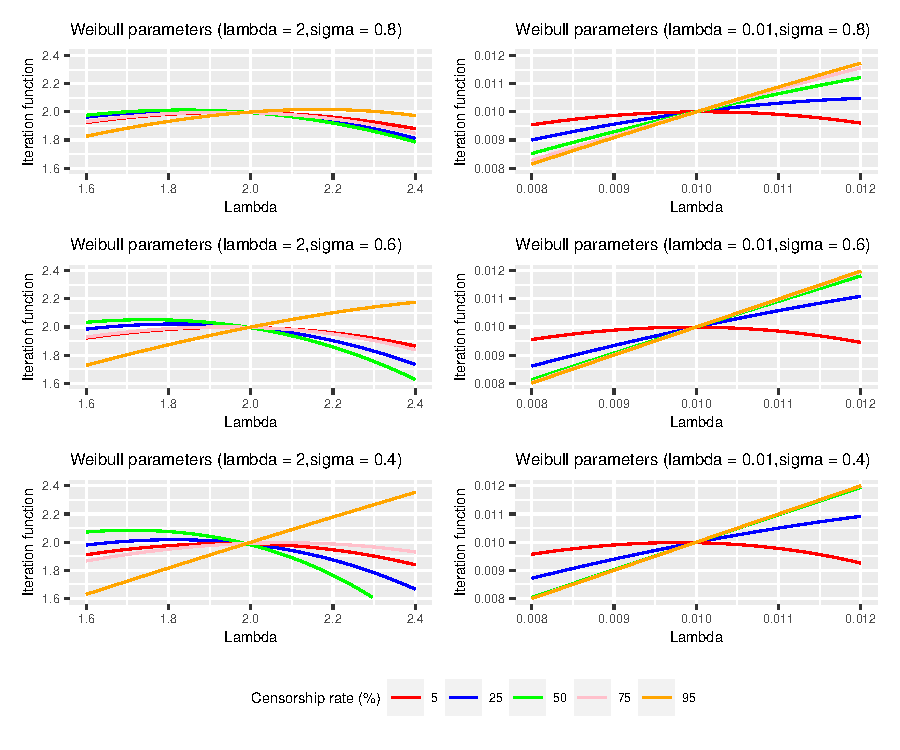
\includegraphics{figs/App/ite_function.pdf}
    \caption{Iteration function plot. The values of $y_i$ used was drawned from a 1000000 size samples of Weibull realisations with parameters $(\lambda^\star,\sigma)$}
    \label{fig:ite_func}
\end{figure}

We also provide in Figure \ref{fig:dll_func} the variations of the second derivative $\partial^2\mathcal{L}(\lambda;y,\sigma)$. We can assume that it is strictly positive as stated in Chapter \ref{chp:4} ensuring the existence of a minimum in the neighbourhood of $\lambda^\star$.  

\begin{figure}[ht]
    \centering
    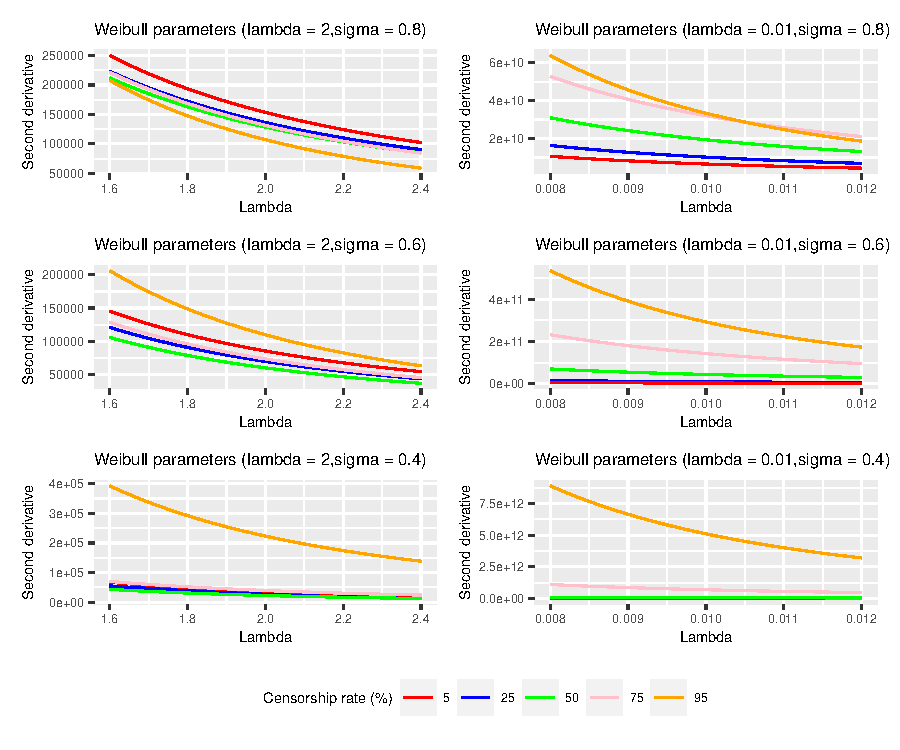
\includegraphics{figs/App/dll_function.pdf}
    \caption{$\partial^2\mathcal{L}(\lambda;y,\sigma)$ plot. The values of $y_i$ used was drawned from a 1000000 size samples of Weibull realisations with parameters $(\lambda^\star,\sigma)$.}
    \label{fig:dll_func}
\end{figure}

\section{Convergence of  \texorpdfstring{$\hat K$}{K} and \texorpdfstring{$\hat t$}{t}}

We provide here the proof of proposition \ref{eq:ml-convergence}. We base our demonstration entirely on the approach developped in \cite{Lavielle1997}. It is assumed that (H1)-(H3) are true. It remains for us to introduce another condition. But first let's denote $\eta_i = \ln f(Y_i,\lambda_{k},\sigma)-\mathbbm{E}[\ln f(Y_i,\lambda_{k},\sigma)]$ for $i$ belonging to the $k$-th segment and associated to the parameters $\lambda_{k}$ and $\sigma$. We have the following proposition: 

\begin{proposition}
     There exists $C < \infty$ such that for any $t\geq 0$ and any $s > 0$,
     \begin{equation}\label{app:C0}
     \mathbbm{E}[\sum_{i=t+1}^{t+s}\eta_i]^2\leq Cs^h,    
     \end{equation}
     for some $1\leq h\leq 2$.
\end{proposition}

This condition corresponds to the condition C0(h) of \cite{Lavielle1997} and is quite common; it is also be found as an assumption in \cite{He2010}. However, it is \cite{Lavielle1997} that gives us the indication that this condition is indeed verified in our case. It explains that in the application framework, if the base signal of $(Y_1,...,Y_n)$ is generated by independent variables, then the variable $\eta_i$ defined in \ref{app:C0} is also a sequence of random variables and the proposition is verified even verified for $h = 1$. Then from Theorem 2.2 of \cite{Lavielle1997}, we have the consistency of the estimator: 
$$ (\hat{\bm \tau}, \hat{\bm \lambda}) \xrightarrow[n\rightarrow \infty]{\PP^{\star}}   (\bm \tau^{\star}, \bm \lambda^{\star})$$

\section{Verifying PELT assumptions}

Some necessary conditions must be met before using the PELT algorithm. It can be found in Theorem 3.1 of \cite{Killick2012} and can be stated as follow:  
\begin{proposition}
    We assume that  when  introducing a changepoint into a sequence of observations the  cost, $\mathcal{C}$, of the sequence reduces. More formally, we assume there exists a constant $K$ such that for all $t<s<T$,
    \begin{equation}\label{app:pelt}
      W(y_{t:s}) + W(y_{s:T}) + K \leq W(y_{t:T})  
    \end{equation}
    Then if
    \begin{equation}\label{app:pelt2}
      F(t)+W(y_{t:s})+K \geq F(s)  
    \end{equation}
    holds, at a future time $T>s$, $t$ can never be the optimal last change point prior to $T$.
\end{proposition}

\textbf{Proof:} The equation \ref{app:pelt} is always verified with working with additive criterion such as the log likelihood. We can see that in the case of our cost function: 
$$W(y_{t:s},\hat\lambda_{t:s})+W(y_{s:T},\hat\lambda_{s:T})+K\leq W(y_{t:T},\hat\lambda_{t:T})$$
It is a direct consequence of using the maximum likelihood estimator. Suppose now that \ref{app:pelt2} is true. Adding $W(y_{s:T},\hat\lambda_{s:T})$ on both sides of the inequation gives : 
\begin{align*}
  F(t)+W(y_{t:s},\hat\lambda_{t:s})+W(y_{s:T},\hat\lambda_{s:T})+K &\geq F(s)+W(y_{s:T},\hat\lambda_{s:T}) \\
  \implies F(t)+W(y_{t:T},\hat\lambda_{t:T}) &\geq F(s)+W(y_{s:T},\hat\lambda_{s:T}),
\end{align*}
We can conclude that the segmentation with the smallest cost is the one with $s$ as the last change-point. So $t$ cannot be the last change-point prior to $T$.

\chapter{Complement of Chapter \ref{chp:5}}

\section{Simulation on the convergence of \texorpdfstring{$\sigma$}{s}} \label{app:sim:chap5}

The experimental protocol is the following. We simulated $N = 100$ samples of size $n = 320$ of left censored Weibull realisations. 3 change points are present in the samples at position $80$, $160$ and $240$. The associated parameters for each segment are $(1,1/100,1/100,1)$. Four scenarios are proposed where the $\sigma^*$ and the censoring rate $\alpha$ varies. We test all configuration possible for $\sigma^* = (0.4,0.8)$ and $\alpha = (25\%,75\%)$. All the results are presented in Figures \ref{fig:sim:sigma1} and \ref{fig:sim:sigma2}.     

\begin{figure}[ht]
    \centering
    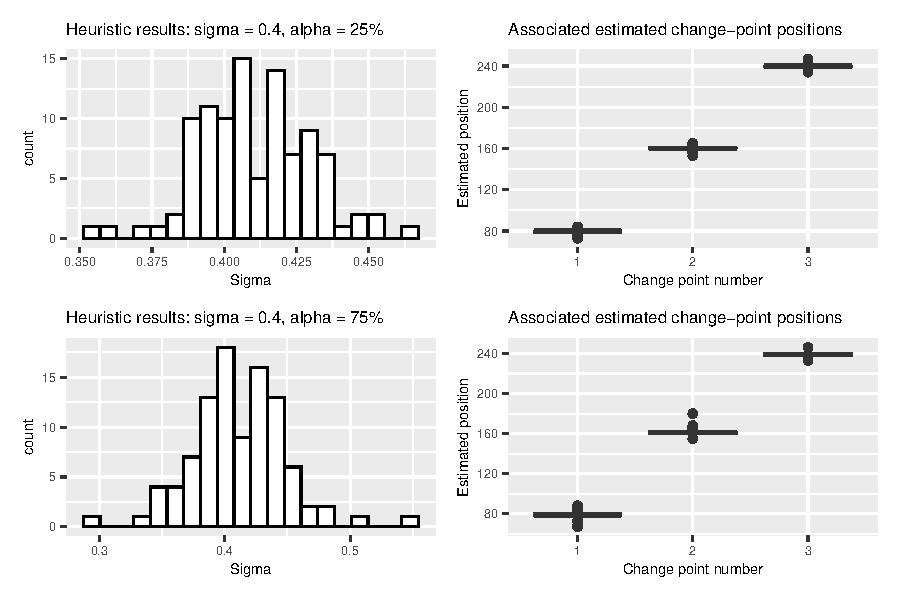
\includegraphics{figs/App/SIM_CHAP5_1.pdf}
    \caption{Scenarios with $\sigma = 0.4$.}
    \label{fig:sim:sigma1}
\end{figure}

\begin{figure}[ht]
    \centering
    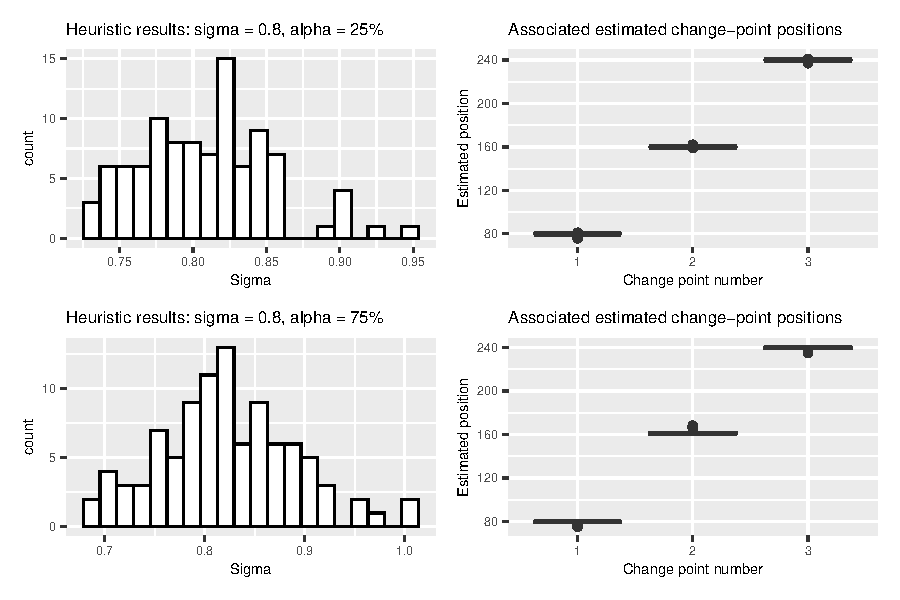
\includegraphics{figs/App/SIM_CHAP5_2.pdf}
    \caption{Scenarios with $\sigma = 0.8$.}
    \label{fig:sim:sigma2}
\end{figure}

For each of these samples, we use the heuristic proposed in \ref{subsection:pelt}. The penalty grid was defined by $Q = 5$ values set to $[\beta_0 = \frac{\ln n}{10},\dots,\beta_{q},\dots,\beta_{Q} = 5\ln n]$ with the $\beta_q$ being equidistant. We allowed this important range in the penalties to ensure enough distinct points for the elbow heuristic. The only PELT parameter that wasn't set as in Chapter \ref{chp:4} was the minimal segment size. It was set to 25. The choice was motivated by the computational time of the simulations, even though we have seen that the estimation of the detection capacity of our method is lower with this minimal segment size. In the procedure, the first iteration $\widehat{\sigma}_0$ is computed with the \texttt{fitdistr} R package \cite{delignette2015}. In the second step of the heuristic, minimizing \ref{new:lk} with respect to $\sigma$ is done using \cite{Byrd1995} which allows for a box constraint for the parameter value $\sigma$ (lower and upper bounds). This interval was set to $[0,1]$. This explains that the estimated values are all inferior to 1 in Figure \ref{fig:sim:sigma2}. We defined a stopping criterion to the heuristic depending on the $\widehat{\sigma}$ values that consists in stopping when the upgrade of the new $\widehat{\sigma}$ is not superior to $10^-3$.

\section{Clustering algorithms}\label{app:clustalgo:chap5}

We keep the same notations than in \ref{subsection:pelt}. We introduce the following new notations : 
\begin{itemize}
    \item $C_m^p$ the $m$-th cluster located in component $p$.
    \item $M_p$ the number of clusters in component $\mathcal{K}_p$.
    \item $\displaystyle Q(\mathcal{K}_p,C_m^p) = \frac{1}{\lvert C_m^p\rvert}\sum_{v_i,v_j \in C_m^p}d_{ij}^2$ the inertia of cluster $C^p_m$.
    \item $\displaystyle R_p(M_p) = \min_{(C_m^p)_{m=1}^{M_p}}\sum_{m = 1}^{M_p}Q(\mathcal{K}_p,C_m^p)$ the best partition (in the sense of minimal inertia) of component $p$ into $M_p$ clusters. 
    \item $\displaystyle S(l,m) = \min_{(M_p)_{p=1}^l \text{ such that } \sum_{p=1}^l M_p = m}\sum_{p=1}^lR_p(M_p)$ which is the best partition of the $l$ first components into a total number of $m$ clusters.
\end{itemize}

$R_p(m)$ can be computed with Ward hierarchical clustering technique. In the case of this work we used the \texttt{R} package \texttt{hclust}. With these notations, we can write the two developed methods as follows: 

\begin{algorithm}[ht]
\caption{Clustering with greedy method:}\label{algo:greed}
\begin{algorithmic}

\State \textbf{input} : the station graph $G=(V,E)$, the known partition into non connex components $(\mathcal{K_1},\dots,\mathcal{K}_P)$, a total number of clusters $M$ \\
  
\State \textbf{initialisation} : Compute $R_p(1)$ for all $p \in [1,\dots,P]$ using \texttt{hclust}, set $M_{opt} = (1,\dots,1)$ vector of size $P$  \\

\For{$m = 1$ to $M-P$}
  \State $\textit{score}\gets(0,\dots,0)$ vector of size $P$
  \For{$p = 1$ to $P$}
  \State $M_{opt}(p) \gets M_{opt}(p) + 1$
  \State $\textit{score}(p) \gets \sum_{p=1}^P R_p(M_{opt}(p))$
  \State $M_{opt}(p) \gets M_{opt}(p) - 1$
  \EndFor
  \State $\textit{pos} \gets which.min(\textit{score})$
  \State $M_{opt}(pos) \gets M_{opt}(pos)+1$
\EndFor
\For{$p=1$ to $P$}
\State built the optimal partition of $\mathcal{K}_p$ with $M_{opt}(p)$ clusters using \texttt{hclust}.
\EndFor

\end{algorithmic}
\end{algorithm} 

\begin{algorithm}[ht]
\caption{Clustering by dynamic programming:}\label{algo:dyn}
\begin{algorithmic}

\State \textbf{input} : the station graph $G=(V,E)$, the known partition into non connex components $(\mathcal{K_1}$, a total number of clusters $M$ \\
    
 \For{$p=1$ to $P$} : 
 \State Use \texttt{hclust} to compute $R_p(m)$ for all $m \in \{1,\dots,M-P+1\}$
 \EndFor 
 \For{$m=1$ to $M-P+1$} : 
 \State $S(1,m) \gets R_1(m)$ 
 \EndFor 
 \For{$l = 2$ to $P$} : 
  \For{$m = l$ to $M$} : 
     \State $W(l,m) \gets 1$ 
     \State $S(l,m) \gets S(l-1,m-1)+R_l(1)$
   \For{$u = 1$ to $m-l+1$}
   \If{$S(l-1,m-u)+R_l(u) < S(l,m)$}
     \State $W(l,m) \gets u$
     \State $S(l,m) \gets S(l-1,m-u)+R_l(u)$
   \EndIf
   \EndFor
 \EndFor 
 \EndFor 
 \State $M_{opt} \gets (\text{NA},\dots,\text{NA})$
 \State $P_{opt}(P) \gets W(P,M)$
 \State $\textit{left} \gets M-W(P,M)$
 \For{$p = P-1$ to $1$}
 \State $P_{opt}(p) \gets W(p,\textit{left})$
 \State $\textit{left} \gets \textit{left}-W(p,\textit{left})$
 \EndFor
 \For{$p = 1$ to $P$}
 \State built the optimal partition of $\mathcal{K}_p$ with $P_{opt}(p)$ clusters using \texttt{hclust}
 \EndFor 
\end{algorithmic}
\end{algorithm} 

\clearpage

\section{Modified empirical Wasserstein distance}\label{appendix:wasserstein}

The Wasserstein distance was chosen over the Kolmogorov-Smirnov or the Jensen-Shannon metric. It has the advantage of integrating in the distance calculation both the differences between the probabilities of observing different values but also the distances between those values. This is a critical point which is illustrated on a simple simulated example provided by Figure \ref{fig:ex_dist}. We show here three monitoring stations that have quite different behaviors. Those different behaviors are obvious both on in the temporal representation and in the histograms. However, the Kolmogorov-Smirnov distance between stations 1 and 3 is equal to the Kolmogorov-Smirnov distance between stations 1 and 2. This distance cannot capture the fact that station 2 recorded higher concentration values than station 3. On the contrary, the Wasserstein distance between stations 1 and 3 is smaller than the Wasserstein distance between stations 1 and 2. 

Computing information theoretic distances/dissimilarities such as the Jensen-Shannon divergence requires estimating densities for the distributions observed at the stations. As noted earlier, few concentration records (and even fewer quantified ones) are available at the level of a station and within a time period. Therefore, density estimations based on such a small number of observations are unreliable.

\begin{figure}[ht]
    \centering
    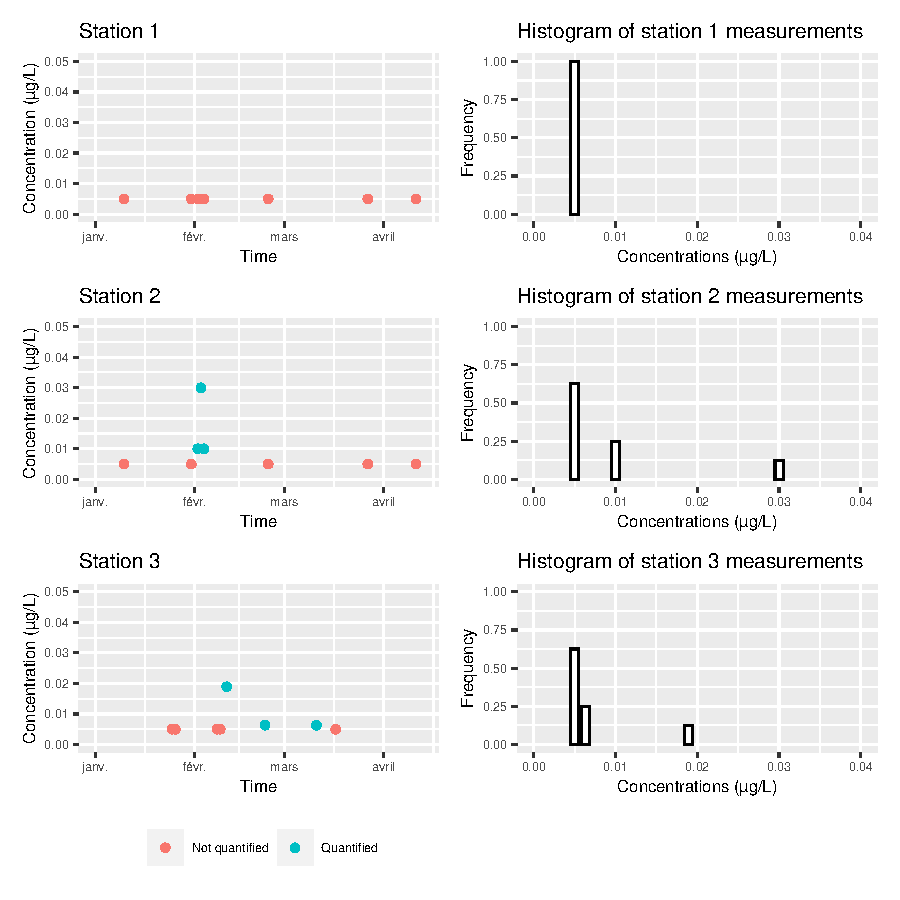
\includegraphics{figs/App/Simu_ex.pdf}
    \caption{Example of three stations data. The data were simulated.}
    \label{fig:ex_dist}
\end{figure}

The empirical 1-d Wasserstein distance used in our work is slightly adapted for left censored values. Given two samples $\bm{x}=(x_1,\dots,x_n)$ and $\bm{y}=(y_1,\dots,y_m)$ of sizes $n$ and $m$ with respective empirical c.d.f. $F_n$ and $G_m$, the 1-d empirical distance writes:
$$W_1(F_n,G_n) = \int_{\mathbbm{R}}\lvert F_n(x)-G_m(x) \rvert\mathrm{d}x$$
In the case of left censored observations, the empirical c.d.f. the first non zero value is the censoring threshold. If we use the classical empirical c.d.f., it does not take into account that the potential real values of censored samples is potentially lower than this threshold. In particular, if both samples $\bm{x}$ and $\bm{y}$ are fully censored at respective thresholds $a_1$ and $a_2$, the Wasserstein distance equals $\lvert a_1-a_2 \rvert$. We would like this quantity to be the smallest possible since none of the samples has any quantified values. Since the samples size for a single station is usually very small, a reasonable assumption is to suppose that the real values under the censoring threshold are uniformly distributed. Figure \ref{fig:mod_dist} illustrates the changes it implies on the empirical c.d.f.. In the previous example of $\bm{x}$ and $\bm{y}$, the adapted empirical distance gives $\lvert a_1-a_2\rvert/2$.    

\begin{figure}[ht]
    \centering
    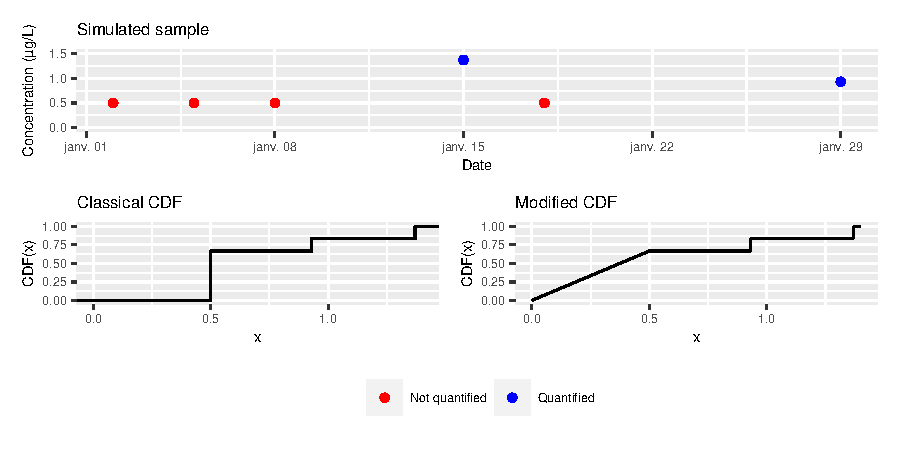
\includegraphics{figs/App/Wass_ew.pdf}
    \caption{Example of modified c.d.f. for the Wasserstein distance.}
    \label{fig:mod_dist}
\end{figure}

\section{Supplementary Figures}

\subsection{Regional map of crops}\label{section:crops}
The regional map of crops provided in Figure \ref{fig:crops} have been produced using data from the \emph{registre parcellaire graphique} produced by the IGN \cite{IGN:RPG}.

\begin{figure}[ht]
    \centering
    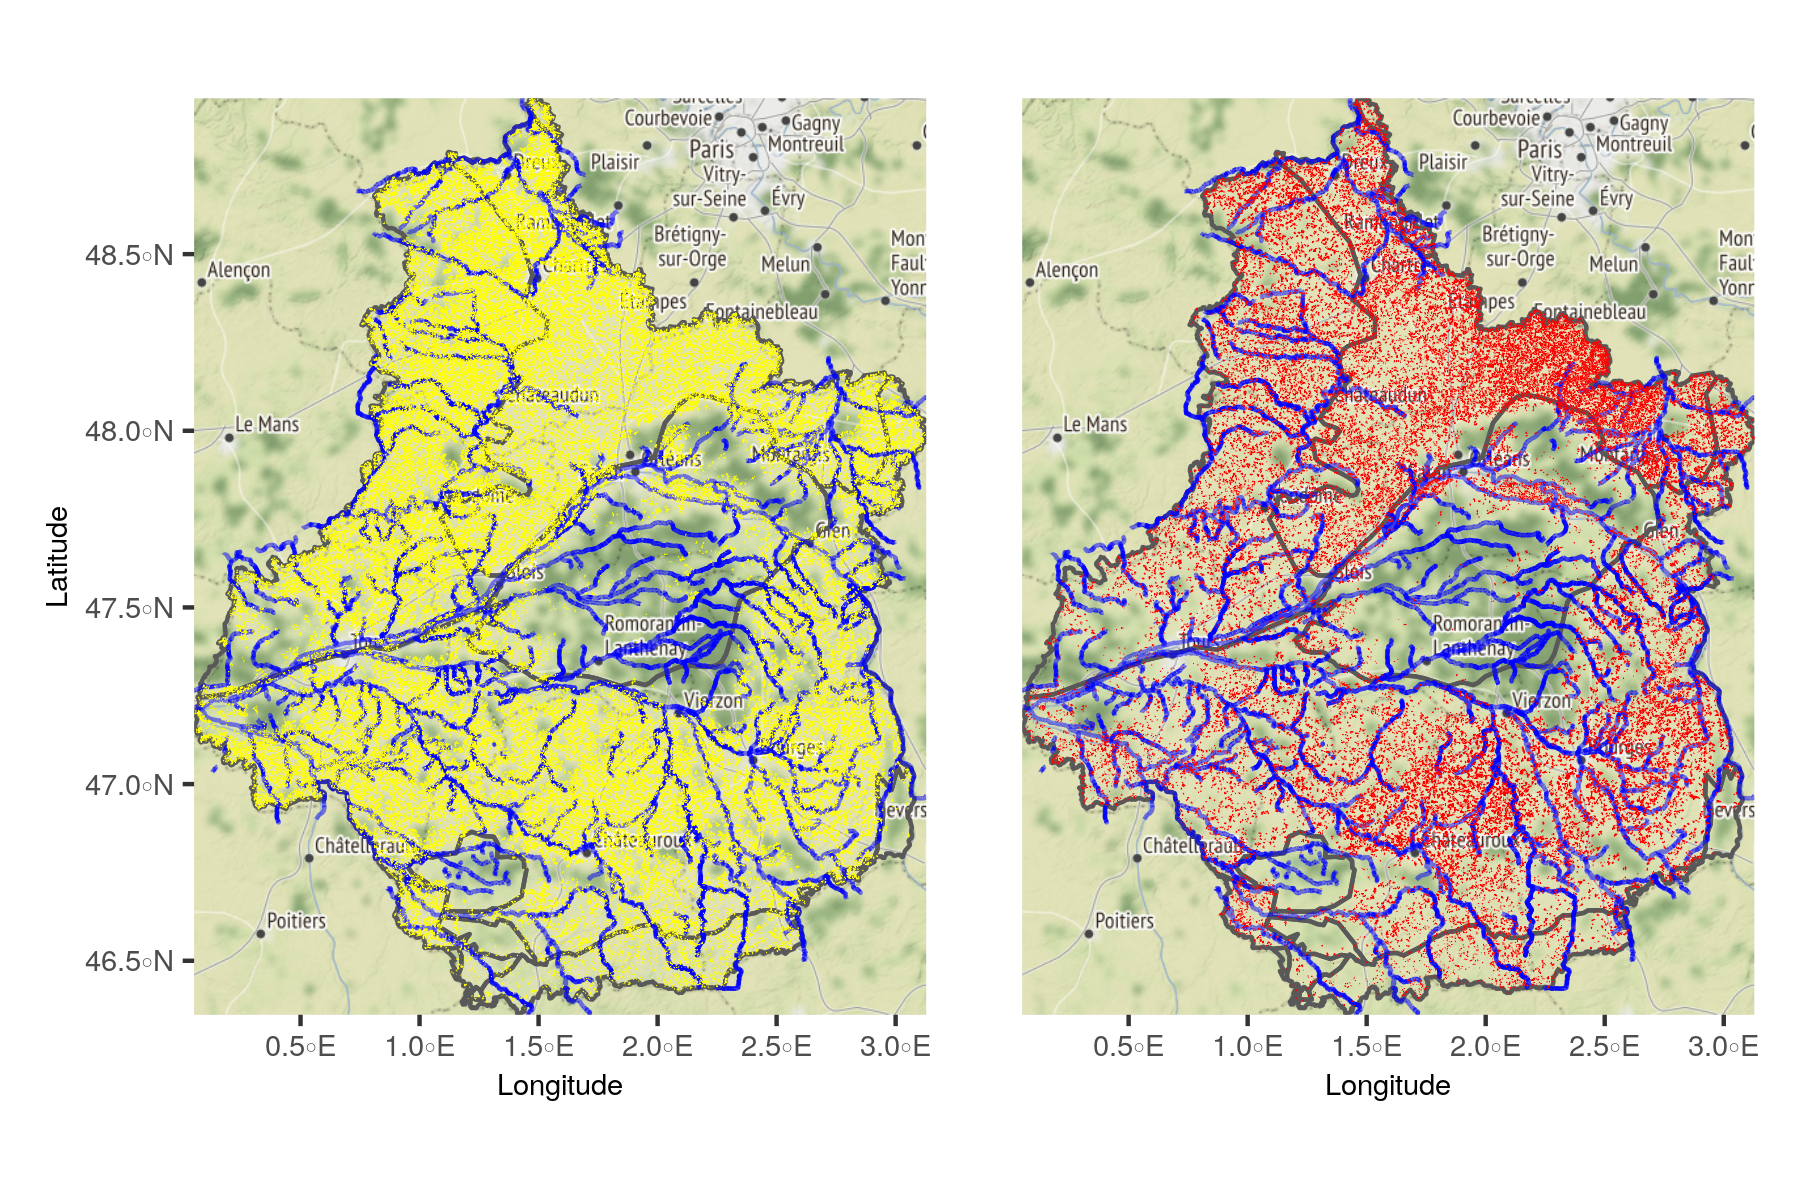
\includegraphics{figs/App/Occ_soil.png}
    \caption{Wheat (in yellow) and barley (in red) crops location in Centre-Val de Loire}
    \label{fig:crops}
\end{figure} 

\subsection{Prosulfocarb sales}\label{section:sale}

Prosulfocarb sales figures used to build Figure \ref{fig:sale} are made available by the \emph{Système d'information sur l'eau} \cite{BNVD}.

\begin{figure}[ht]
  \centering
  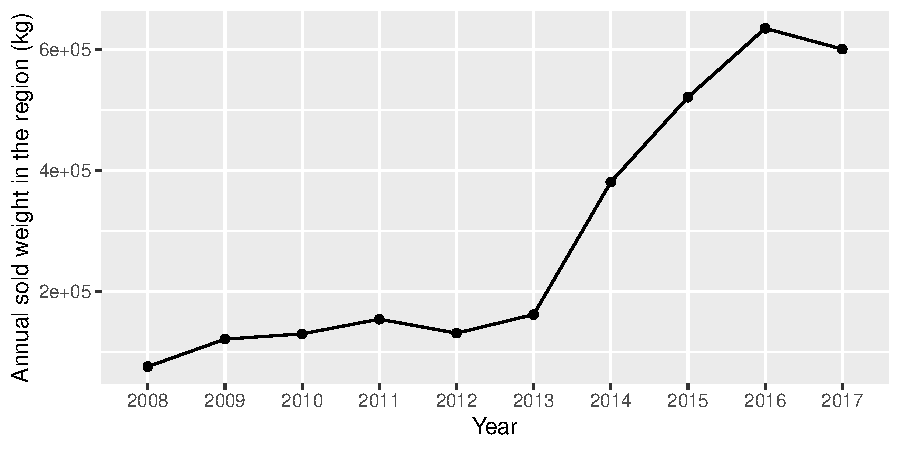
\includegraphics[]{figs/App/Sales_pro.pdf}
  \caption{Prosulfocarb sales between 2008 and 2017 in the Centre-Val de Loire region}
  \label{fig:sale}
\end{figure}

\subsection{All elbow methods figures}\label{section:elb}

\begin{figure}[ht]
  \centering
  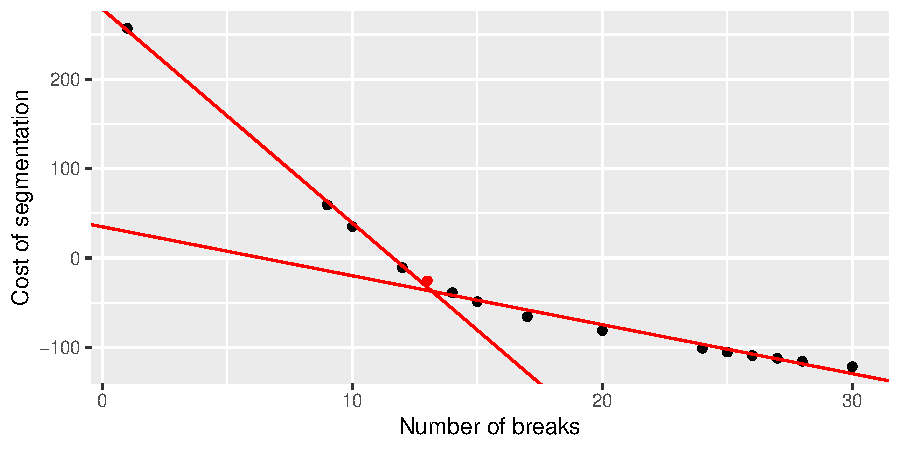
\includegraphics[]{figs/App/Elbow_seg.pdf}
  \caption{Elbow method selecting the optimal segmentation of the full signal $\overline{\mathcal{D}}$.}
  \label{fig:elb_seg}
\end{figure}

\begin{figure}[ht]
  \centering
  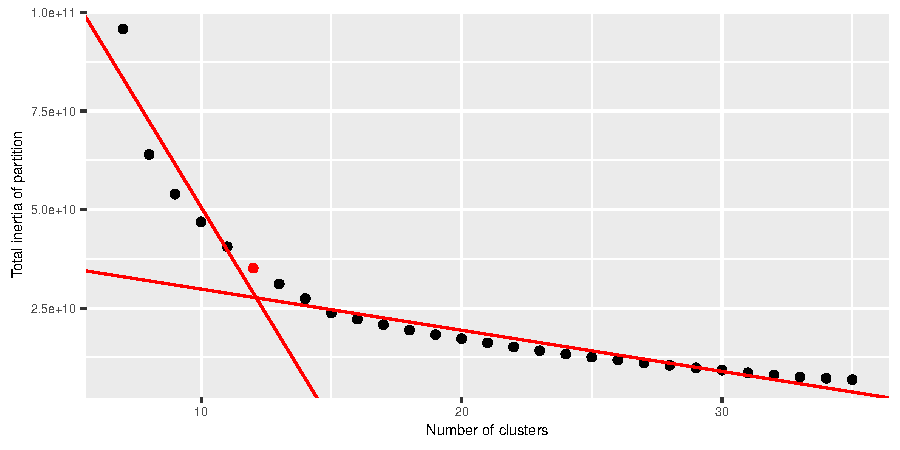
\includegraphics[]{figs/Chap5/Elb_clust.pdf}
  \caption{Elbow method for the spatial clustering.}
  \label{fig:elb:clust}
\end{figure}
\end{appendices}